\section{Translator Architecture}

\begin{figure}[htp]
  \centering
  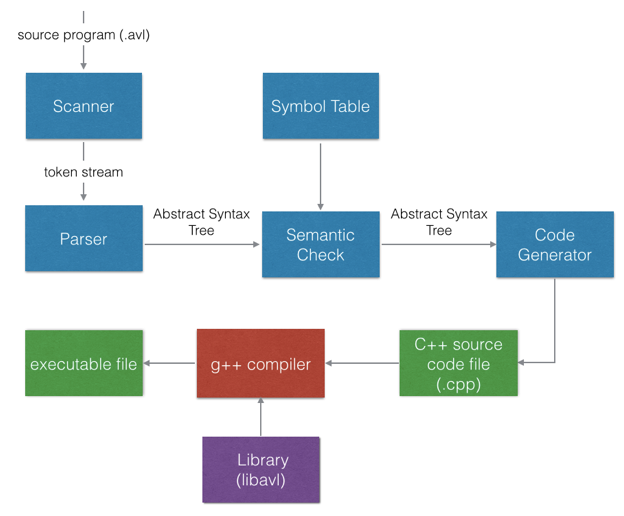
\includegraphics[height=12cm]{architecture.png}
  \caption{Translator architecture}
  \label{fig:arch}
\end{figure}

\subsection{Scanner}
The string of source code, from .avl file, is passed into Scanner, which continuously groups
characters into lexemes, and outputs tokens. Jiuyang Zhao firstly drafted the scanner, and the
entire team contribute to the final version.

\subsection{Parser}
Our grammar is written in the parser. It uses tokens produced by the scanner to create an abstract
syntax tree, which depicts the grammatical structure of the token stream. Augmented by the SDD, the
parser generated an AST during evaluating token stream. This AST is consisted of nodes, which has
type and value. Qianxi Zhang and Jiuyang Zhao deliberated the grammar. Qianxi Zhang and Yu Zheng
implemented the SDD. Finally the entire team validated it consistent with the LRM.

\subsection{Symbol Table}
The entire program has a linked list of symbol tables, one per scope. Each identifier has a
corresponding entry in the symbol table. Hash value of the identifier name is used as the key. The
symbol table was written Qinfan Wu and refined by the entire team.

\subsection{Semantic Check}
The semantic analyzer uses the AST and the information in the symbol table to check the source
program for semantic consistency with the language definition. In this phase, we do scope checking
and validation on semantics. For a running program, there is a stack storing scope-directed symbol
tables. To validate a function call, we search it in the symbol table at the bottom of the stack. To
validate a variable, we search it from the top of the stack. If no symbol table contains it, an
error is reported. Shining Sun implemented this part.

\subsection{Code Generator}
For the purpose of easily debugging, we separate semantic check from code generator. It takes the
AST generated by the parser as input. While traversing the tree, the generator produces C++ code, by
parsing each node. It outputs the C++ code to a .cpp file. The generator was initially written by
Qianxi Zhang, and the entire team gave feedback and refined to the final version.

\subsection{Library (libavl)}
The “libavl” is a shared library, which is used for supporting visualization. It defines different
data types and visualizers in order to use OpenGL to do visualization. The translated C++ code is
linked with libavl, and then passed to C++ compiler, which generates an executable file. This
library architecture was written by Qinfan Wu, Shinig Sun, and Yu Zheng.

All of the above modules are grouped together and run by automake, which was written by our System
Integrator Qinfan Wu.
